\documentclass[class=report,crop=false, 12pt]{standalone}
\usepackage[screen,nosolutions]{../myscratch}
%\usepackage[screen]{../myscratch}


\begin{document}

\titre[S]{Listes}
%===============================


\insertvideo{Evt1pIm91O8}{Listes -- Activité 1}

\insertvideo{Kl3hdt1CrGU}{Listes -- Activité 2}

\insertvideo{bG7Y4JUn-c0}{Listes -- Activité 3}

\bigskip
\bigskip

\begin{activite}[Calcul de la moyenne]

Écris un programme qui demande trois notes à l'utilisateur et ensuite en calcule la moyenne.

\begin{center}
  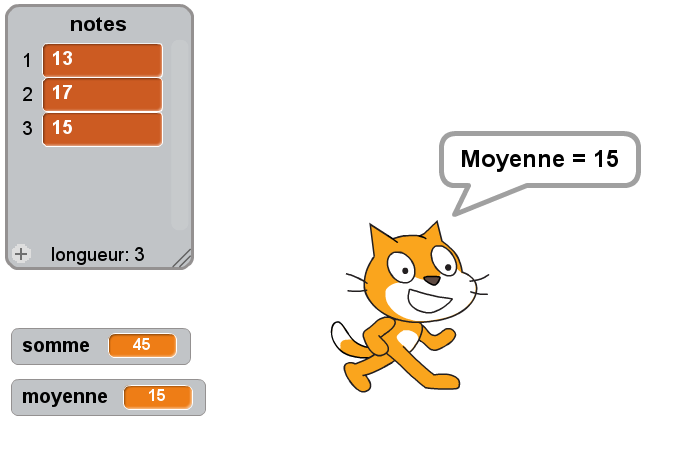
\includegraphics[width=0.8\textwidth]{ecran-12-ex1} 
\end{center}

\begin{itemize}
  \item Crée une liste \codeinline{notes}.
  \item Demande trois notes à l'utilisateur. Ajoute chaque note à la liste.
    
  \item Calcule la somme des trois notes. Pour cela :
  \begin{itemize}
    \item Crée une variable \codeinline{somme} initialisée à $0$.
    
    \item Crée une variable \codeinline{n} initialisée à $0$. Ce sera le \emph{compteur} pour parcourir la liste. 
    
    \item Répète $3$ fois : ajouter $1$ à \codeinline{n} ; ajouter à
    \codeinline{somme} l'élément numéro \codeinline{n} de la liste \codeinline{notes}.    
  \end{itemize}
  
  \item La moyenne s'obtient par la formule :
  $$\text{moyenne} = \frac{\text{somme des notes}}{\text{nombre de notes}}$$
\end{itemize}


\bigskip

\textbf{Bonus.}
\begin{itemize}
  \item Modifie ton programme de sorte que le nombre de notes soit une variable. 
  
  \item Tu peux même demander à l'utilisateur de combien de notes il souhaite calculer la moyenne.
  
\end{itemize}

\bigskip

\textbf{Blocs utiles.}

\begin{itemize}
  \item On crée une liste à partir de la catégorie \og Données \fg{}. Ici la liste \codeinline{notes} contiendra trois nombres.
  
 
  \item On ajoute les éléments un par un. Par exemple, voici le bloc pour ajouter la note $15$ à la liste.
\begin{center}
\ovallist{notes}
\qquad\qquad\qquad
\begin{scratch}
  \blocklist{ajouter \ovalnum{15} à \selectmenu{notes}}
\end{scratch}
\end{center} 

  \item On peut récupérer un élément de la liste. Par exemple, voici comment récupérer le premier élément ainsi que celui en position $n$
  ($n$ est notre compteur qui peut valoir $1$, $2$, $3$...).
\begin{center}
  \ovallist{élément \ovalnum{1} de \selectmenu{notes}}
  \qquad\qquad\qquad
  \ovallist{élément \ovalvariable{n} de \selectmenu{notes}}
\end{center}   
  \item Pour démarrer à chaque fois en partant d'une liste vide, commence ton programme avec le bloc :
\begin{center}
\begin{scratch}
  \blocklist{supprimer tous les éléments de la liste \selectmenu{notes}}
\end{scratch}
\end{center}   
\end{itemize}

\end{activite}




\begin{activite}[Le cadavre exquis]

Programme un jeu de mots : forme une phrase au hasard à partir d'un sujet, d'un verbe, d'un lieu et d'un complément.

\begin{center}
  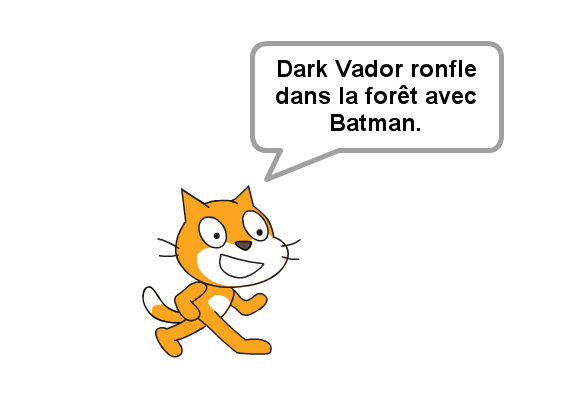
\includegraphics[width=0.6\textwidth]{ecran-12-ex2} 
\end{center}

\begin{itemize}
  \item Crée une liste de sujets (par exemple : \codeinline{sujets} = [Le chat, Dark Vador, Ma voisine, Mickey Mouse,...]).
  \item Crée une liste de verbes (par exemple : [mange, plonge, ronfle, grimpe,...]).
  \item Crée une liste de lieux (par exemple : [dans la piscine, dans la forêt, à la plage, sur la neige,...]).  
  \item Crée une liste de compléments (par exemple : [avec plaisir., sans s'arrêter., en boudant., avec Batman.,...]). 
  \item Crée une variable \codeinline{monsujet} qui stocke un élément au hasard de la liste des sujets, idem avec un verbe, un lieu et un complément.
  \item Affiche une phrase composée de ce sujet, ce verbe, ce lieu et ce complément.
\end{itemize}



\bigskip

\textbf{Blocs utiles.}
Voici une petit programme qui tire au hasard un élément d'une liste et l'affiche : on tire au hasard un entier $n$ (entre $1$ et le nombre total d'éléments dans la liste), puis on affiche l'élément de rang $n$.

\begin{center}
\begin{scratch}
  \blockinit{quand \greenflag est cliqué}
  \blockrepeat{répéter \ovalnum{10} fois}
  {
    \blockvariable{mettre \selectmenu{n} à \ovaloperator{nombre aléatoire entre \ovalnum{1} et \ovallist{longueur de \selectmenu{maliste}}}}
    \blocklook{dire  
     \ovallist{élément \ovalvariable{n} de \selectmenu{maliste}} pendant \ovalnum{2} secondes}    
  }
\end{scratch}
\end{center} 
  
\end{activite}




\begin{activite}[Le loto en couleur]

Programme un mini-jeu de loto en couleur.
\begin{itemize}
  \item Une urne contient $6$ boules : 3 noires, 2 rouges, 1 bleue.
  \item On tire au hasard une première boule (puis on la remet dans l'urne) ; on tire au hasard une seconde boule (puis on la remet dans l'urne).
  \item C'est gagné si l'une des boules est rouge et que l'autre est bleue.
  \item Répète $10\,000$ tirages. Sur ces $10\,000$ tirages, combien en obtiens-tu de gagnants ?
\end{itemize}

\bigskip

\emph{Indications.} 
\begin{itemize}
  \item Crée une liste [N,N,N,R,R,B] qui modélise les boules de l'urne. 
  \item Attention, il n'y a pas d'ordre. Le tirage (R,B) et le tirage (B,R) sont tous les deux gagnants !
\end{itemize}
  
\end{activite}




\ifx \displaysolutions \myzero
\else
\begin{code}
\setscratch{scale=\scalesolution}
\onesolution{Listes}{Activité 1}{
\begin{scratch}
  \blockinit{quand \greenflag est cliqué}
  \blocklist{supprimer tous les éléments de la liste \selectmenu{notes}}
  \blockvariable{mettre \selectmenu{nbnotes} à \ovalnum{3}}
  \blockrepeat{répéter \ovalvariable{nbnotes} fois}
  {
    \blocksensing{demander \ovalnum{Une note ?} et attendre}
    \blocklist{ajouter \ovalsensing{réponse} à \selectmenu{notes}} 
  }
  \blockvariable{mettre \selectmenu{somme} à \ovalnum{0}}
  \blockvariable{mettre \selectmenu{n} à \ovalnum{0}}
  \blockrepeat{répéter \ovalvariable{nbnotes} fois}
  {
    \blockvariable{ajouter \ovalnum{1} à \selectmenu{n}} 
    \blockvariable{ajouter \ovallist{élément \ovalvariable{n} de \selectmenu{notes}} à \selectmenu{somme}}  
  }
  \blockvariable{mettre \selectmenu{moyenne} à \ovaloperator{\ovalvariable{somme} / \ovalvariable{nbnotes} }}
  \blocklook{dire \ovaloperator{regrouper \ovalnum{Moyenne = } et \ovalvariable{moyenne}}}
\end{scratch}
}
\onesolution{Listes}{Activité 2}{
\begin{minipage}{0.62\textwidth}
\begin{scratch}
  \blockinit{quand \greenflag est cliqué}
  \blocklist{supprimer tous les éléments de la liste \selectmenu{sujets}}
\end{scratch}

\smallskip

\hbox{Idem pour verbes, lieux, complements}

\bigskip

\begin{scratch}
    \blocklist{ajouter \ovalnum{Le chat} à \selectmenu{sujets}}
    \blocklist{ajouter \ovalnum{Dark Vador} à \selectmenu{sujets}}
\end{scratch}

\smallskip

\hbox{Etc.}

\bigskip

\begin{scratch}
  \blockvariable{mettre \selectmenu{n1} à \ovaloperator{nombre aléatoire entre \ovalnum{1} et \ovallist{longueur de \selectmenu{sujets}}}}
  \blockvariable{mettre \selectmenu{monsujet} à \ovallist{élément \ovalvariable{n1} de \selectmenu{sujets}}}
  \blockvariable{mettre \selectmenu{n2} à \ovaloperator{nombre aléatoire entre \ovalnum{1} et \ovallist{longueur de \selectmenu{verbes}}}}
  \blockvariable{mettre \selectmenu{monverbe} à \ovallist{élément \ovalvariable{n2} de \selectmenu{verbes}}}
  \blockvariable{mettre \selectmenu{n3} à \ovaloperator{nombre aléatoire entre \ovalnum{1} et \ovallist{longueur de \selectmenu{lieux}}}}
  \blockvariable{mettre \selectmenu{monlieu} à \ovallist{élément \ovalvariable{n3} de \selectmenu{lieux}}}
  \blockvariable{mettre \selectmenu{n4} à \ovaloperator{nombre aléatoire entre \ovalnum{1} et \ovallist{longueur de \selectmenu{complements}}}}
  \blockvariable{mettre \selectmenu{moncomplement} à \ovallist{élément \ovalvariable{n4} de \selectmenu{complements}}}
  \blockvariable{mettre \selectmenu{phrase} à 
        \ovaloperator{regrouper \ovalvariable{monsujet} et 
           \ovaloperator{regrouper \ovalvariable{monverbe} et 
              \ovaloperator{regrouper \ovalvariable{monlieu} et \ovalvariable{moncomplement}} }}}
  \blocklook{dire \ovalvariable{phrase}}
\end{scratch}
\end{minipage}
}
\onesolution{Listes}{Activité 3}{
\begin{scratch}
  \blockinit{quand \greenflag est cliqué}
  \blocklist{supprimer tous les éléments de la liste \selectmenu{boules}}
  \blocklist{ajouter \ovalnum{N} à \selectmenu{boules}}
  \blocklist{ajouter \ovalnum{N} à \selectmenu{boules}}
  \blocklist{ajouter \ovalnum{N} à \selectmenu{boules}}
  \blocklist{ajouter \ovalnum{R} à \selectmenu{boules}}
  \blocklist{ajouter \ovalnum{R} à \selectmenu{boules}}
  \blocklist{ajouter \ovalnum{B} à \selectmenu{boules}}
  \blockvariable{mettre \selectmenu{bonstirages} à \ovalnum{0}}
  \blockrepeat{répéter \ovalnum{10000} fois}
  {
    \blockvariable{mettre \selectmenu{n1} à \ovaloperator{nombre aléatoire entre \ovalnum{1} et \ovallist{longueur de \selectmenu{boules}}}}
    \blockvariable{mettre \selectmenu{boule1} à \ovallist{élément \ovalvariable{n1} de \selectmenu{boules}}}
    \blockvariable{mettre \selectmenu{n2} à \ovaloperator{nombre aléatoire entre \ovalnum{1} et \ovallist{longueur de \selectmenu{boules}}}}
    \blockvariable{mettre \selectmenu{boule2} à \ovallist{élément \ovalvariable{n2} de \selectmenu{boules}}}
    \blockif{si \booloperator{\booloperator{\ovalvariable{boule1} = \ovalnum{R}} et \booloperator{\ovalvariable{boule2} = \ovalnum{B}} } alors }
    {
    \blockvariable{ajouter \ovalnum{1} à \selectmenu{bonstirages}} 
    }
    \blockif{si \booloperator{\booloperator{\ovalvariable{boule1} = \ovalnum{B}} et \booloperator{\ovalvariable{boule2} = \ovalnum{R}} } alors }
    {
    \blockvariable{ajouter \ovalnum{1} à \selectmenu{bonstirages}} 
    }
  }
  \blocklook{dire \ovalvariable{bonstirages}}
\end{scratch}
}    
\end{code}
\fi

\end{document}
